\chapter{Symbolic Client Behavior Verification}
\label{ch:scbv}

\newcommand{\execTrace}[1]{\ensuremath{\mathrm{T}_{#1}}\xspace}
\newcommand{\program}[1]{\ensuremath{\mathrm{P}_{#1}}\xspace}
\newcommand{\server}[1]{\ensuremath{\mathrm{S}_{#1}}\xspace}
\newcommand{\clockTrace}[1]{\ensuremath{\mathrm{C}_{#1}}\xspace}
\newcommand{\memoryTrace}[1]{\ensuremath{\mathrm{V}_{#1}}\xspace}
\newcommand{\replayLog}[1]{\ensuremath{\mathrm{R}_{#1}}\xspace}
\newcommand{\lang}[1]{\ensuremath{\mathrm{L}_{#1}}\xspace}
\newcommand{\msgLang}[1]{\ensuremath{\mathrm{L}_{M}}\xspace}
\newcommand{\machine}[1]{\ensuremath{{\Lambda}_{R#1}}\xspace}
\newcommand{\symMachine}[1]{\ensuremath{\mathrm{\Lambda}_{SE#1}}\xspace}
\newcommand{\messageTrace}[1]{\ensuremath{\mathrm{M}_{#1}}\xspace}
\newcommand{\messageTraceAlt}[1]{\ensuremath{\mathrm{\hat{M}_{#1}}}\xspace}

For our purposes, we abstract the client behavior verification
problem as follows. A server wishes to verify that a
client is running the sanctioned software, but does so without
modifying the client (e.g., by having the client send its inputs to
the server).  It therefore has no direct access to client state: the
server knows only its own state and the network messages, that have
been sent and received by the client.

\subsubsection {Ignore This Section Maybe}

The problem can then be
phrased as: \emph{Given a client program P, is it possible for P to
yield output $M$?}  This is illustrated in \figref{fig:intro:prob}.

\begin{figure}[t]
\centering
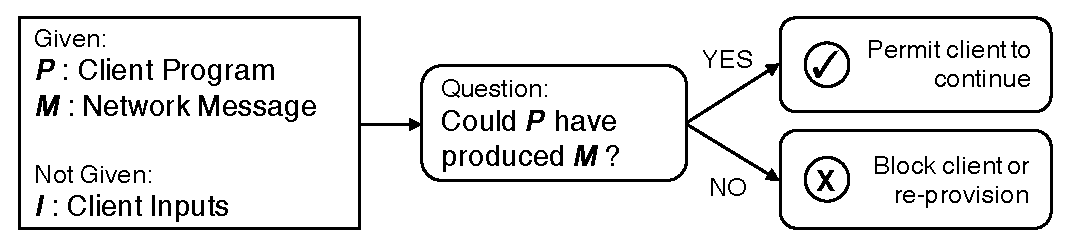
\epsfig{file=figures/introduction/problem.eps, width=0.8\columnwidth}
\caption{Abstracted Client Verification Problem}\label{fig:intro:prob}
\end{figure}

Unfortunately, the general problem of determining whether an arbitrary
program \emph{P} can produce an output \emph{M} is undecidable. 
%Not surprisingly, all current methods for client verification are either
%slow, inaccurate (verify only a model of the client, not the exact
%client executable), probabilistic (with hard-to-gauge error rates), or
%require alterations to the client implementation.
%%\cite{vikram09:ripley,giffin02:remote,guha09:ajax,wagner02:mimicry}.
Fortunately, even though the general problem is undecidable, a
particular instance can be tractable.  

In fact, Cochran and Reiter built a tool (using the KLEE symbolic
execution engine \cite{cadar08:klee}) and demonstrated it on the game
clients for the 2D games Tetrinet and XPilot.  In these two games,
the tool can give a ``Yes'' answer quickly enough to verify
legitimate gameplay in speeds approaching real time.  The ``No''
answer may be slow, but since client is cheating, such a slowdown is
acceptable.

To definitively conclude that a sequence of client messages is
impossible (the uncommon case), our algorithm incurs a cost similar to
Bethea et al.'s~\cite{bethea11:games}, however.  As such, we expect
our algorithm to be useful primarily as an online data reduction
technique that prunes the client messages that must be logged for
offline analysis by that (or another) technique.  In addition, clients
whose messages are not verified quickly by our technique can be
serviced only provisionally (e.g., with fewer privileges and/or
logging to enable undoing their effects) while their verification is
completed offline.


\begin{definition}
  An execution trace \execTrace{} is a sequence of machine or
  bytecode instructions.
\end{definition}

%\begin{definition}
%  A language \lang{P} presents the set of all execution
%  traces \execTrace{} that may be generated by some program $P$.
%\end{definition}

It is generally not feasible to represent \lang{P}, so 
existing techniques build a determine if an execution trace \execTrace{} 
fits a model 

\subsubsection{ This section is good I think}

\begin{definition}
  We define a message trace  as a sequence of messages $\msg{0},
  \msg{1}, \ldots$ corresponding to calls to network send and receive
  events in some client program \program{} communicating with a server
  program. In other words, a message trace contains messages that
  were either sent from the client to the server ore sent from the
  server to the client. The messages are ordered from client's
  perspective.
\end{definition}

\begin{definition}
  A language \msgLang{\program{}} presents the set of all possible message
  traces \messageTrace{} that can be observed, from the client's
  perspective, during a client-server
  session.
\end{definition}

%\begin{definition}
We define client behavior verification as a decision procedure that
takes as input; a program \program{} and a message trace $\msg{0},
\msg{1}, \ldots$ \msg{\msgNmbr}, and outputs if the message trace is
is consistent with \program{}.
A message trace is consistent with a client program \program{} if it
exists in a language  \msgLang{\program{}}, where \msgLang{\program{}}
is the set of all messages traces that could be generated by a client
program \program{} communicating with some server.
%\end{definition}

In this security model, an attacker may only submit messages that as
part of a message trace that exists in \msgLang{\program}. This model
reduces the power of the attacker, but does not guarantee
that there does not exist an attack message trace $\messageTraceAlt{}
\in \msgLang{\program{}}$. However, it severely reduces the power of
the attacker to only generating messages that are indistinguishable
from a valid client.

Enumerating \msgLang{\program{}} in the general
case is not feasible, but we show this dissertation that client
behavior verification can be achieved by either bounding the size of
the number of execution paths in a client program or by generating an
execution trace, that can be used to show that a message trace is 
is contained within \msgLang{\program{}}.
These two approaches to client behavior verification have different
requirements and limitations and the remainder of this dissertation
will consist of a description of these techniques and evaluations on
case study applications. In \chref{ch:scv}, we determine if a message
trace is in \msgLang{\program} incrementally, using symbolic
constraints, generated by executing a subset of paths in a modified
version of the client program. These accumulated constraints represent
a subset of \msgLang{\program}. Our second approach, described in
\chref{ch:guided} and extended in \chref{ch:par}, searches for a
possible execution trace (sequence of client instructions) that can be
used to show that a message trace is a member of \msgLang{\program}.

\subsubsection{ Ignore this section Maybe also}

\begin{definition}
  An execution trace \execTrace{} is a sequence of machine or
  bytecode instructions.
\end{definition}

\begin{definition}
  A language \lang{P} presents the set of all execution
  traces \execTrace{} that may be generated by some program $P$.
\end{definition}

\begin{definition}
  An replay log is a tuple $\replayLog{} = (\execTrace{},
  \memoryTrace{} )$ where \execTrace{} is a execution
  trace and \memoryTrace{} is a set of values such that
  $|\execTrace{}| = |\memoryTrace{}|$. The ith
  instruction in \execTrace{} occurred at time equal to the ith time
  in \clockTrace{} and if it was a memory load, the instruction loaded
  the value in \memoryTrace{}. A replay log can be used to replay an
  execution precisely, including any values that were read from
  hardware, such as random numbers or interrupt driven inputs (e.g.,
  keyboard or mouse).
\end{definition}

\begin{definition}
  A procedure \machine{} is a program that takes as input
  a replay log \replayLog{}, replays each tuple in \replayLog{}
  and emits a message trace \messageTrace{} representing all
  calls to \posixSend and \posixRecv in the execution trace.
\end{definition}

\begin{definition}
  Replay client verification is a decision procedure that takes as
  input, a program \program{}, a replay log \replayLog{} and a message
  trace \messageTrace{} and outputs valid if the execution trace
  \execTrace{} is in \lang{\program{}} and
  $\machine{}(\replayLog{})$ emits a \messageTraceAlt{} such that
  $\messageTraceAlt{} = \messageTrace{}$.
\end{definition}

Under replay client verification, all clients must submit a replay log
to the server at the end of a session. This way, a server can verify 
a client's message trace, without enumerating all members of
\msgLang{\program}. This model is equivalent to client verification.

We implement the client behavior decision procedure using symbolic
execution. One could conceivably use symbolic execution to 

\begin{definition}
  A procedure \symMachine{} is a program that takes as input
  an execution trace \execTrace{} and uses symbolic execution
  to replay \execTrace{}, using symbolic values for any loads from
  uninitialized memory and 
  emits a symbolic message trace \messageTrace{}
  and associated conditions for each of the branch instructions in
  \execTrace{}.
\end{definition}

\begin{definition}
  Symbolic client verification is a decision procedure that takes as
  input, a program \program{}, a execution trace \execTrace{} and a message
  trace \messageTrace{} and outputs valid if the execution trace
  \execTrace{} is in \lang{\program{}} and
  $\symMachine{}(\replayLog{})$ emits a \messageTraceAlt{} such that
  $\messageTraceAlt{} = \messageTrace{}$ is satisfiable.
\end{definition}

Under symbolic client verification, no additional demands are
made on the client. 

\begin{definition}
  An execution prefix \execPrefix{} is a prefix of an execution
  trace \execTrace{} that is valid according to symbolic client
  verification for a prefix of some  message trace \messageTrace{}.
\end{definition}

\section{Server-side Program Anomaly Detection}
A common defense against attackers is program anomaly detection.
Program anomaly detection analyzes program behavior and determines
whether the execution of a program is behaving as expected under
normal operation. There are numerous approaches... The server software
is monitored to generate an \execTrace{} for 

